\documentclass[tikz]{standalone}
\usepackage{tikz,amsmath}
\usetikzlibrary{shapes}
\begin{document}
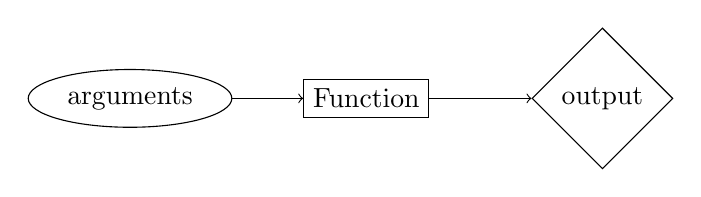
\begin{tikzpicture}
    \node (A) [rectangle, draw] at (0, 0) {Function};
    \node (B) [ellipse, draw] at (-3, 0) {arguments};
    \node (D) [diamond, draw] at (3, 0) {output};
    \draw [->] (B) -- (A);
    \draw [->] (A) -- (D);
\end{tikzpicture}
\end{document}
